\section{Método del gradiente conjungado}

\subsection{Problema}

Dada $A \in \mathbb{R}^{n \times n}$ simétrica definida positiva, queremos calcular la única solución del sistema lineal $Ax = b$.

La idea que usaremos es la siguiente. Consideraremos una función $Q : \mathbb{R}^{n} \to \mathbb{R}$ que alcanza el mínimo absoluto en la solución $A^{-1}b$ del sistema dado. Comenzando con un punto cualquiera sobre el gráfico de $Q$, vamos a movernos en una dirección dada, una cierta distancia, acercándonos al mínimo. Repetimos este proceso sucesivas veces hasta llegar al mínimo.

La función $Q$ que consideraremos no es cualquiera entre las que tienen un mínimo absoluto en $A$. Para poder asegurar que siempre que nos movamos estemos acercándonos al mínimo queremos que el gráfico de $Q$ sea un paraboloide cóncavo.


\begin{figure}[h]
\centering
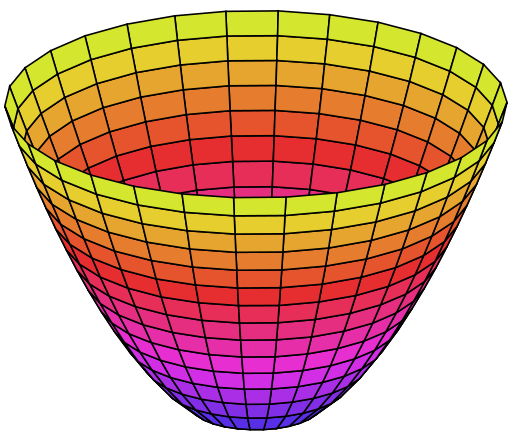
\includegraphics[scale=0.30]{imagenes/paraboloide.png}
\end{figure}

\subsection{El método}

Definimos

\[Q(x) = x^tAx - 2x^tb\]

Como $A$ es simétrica definida positiva, $Q$ resulta tener la forma deseada y además alcanza su mínimo absoluto en $x = A^{-1}b$. Para ver esto último notemos que podemos reescribir $Q(x) = (A^{-1}b - x)^t A (A^{-1}b - x) - b^{t}A^{-1}b$. Como $A$ es definida positiva entonces $(A^{-1}b - x)^t A (A^{-1}b - x) \geq 0$, con lo cual $Q(x) \geq -b^t A^{-1}b$. Luego $Q$ alcanzará el mínimo $-b^t A^{-1}b$ si y sólo si $(A^{-1}b - x)^t A (A^{-1}b - x) = 0 \Leftrightarrow A^{-1}b - x = 0$, nuevamente debido a que $A$ es definida positiva.

Fijemos un punto inicial $x^{(0)} \in \mathbb{R}^n$ y recorramos en dirección $d^{(0)} \in \mathbb{R}^n$ una cierta distancia dada por $\alpha_0 \in \mathbb{R}$, definiendo así un nuevo punto $x^{(1)} = x^{(0)} + \alpha_0 d^{(0)}$. Con este mismo razonamiento definimos una sucesión $\{x^{(k)}\}_k$ que es tal que

\[x^{(k + 1)} = x^{(k)} + \alpha_{k}d^{(k)}\]

Supongamos que la dirección $d^{(k)}$ está fija y es no nula, y miremos $Q(x^{(k + 1)}) = Q(x^{(k)} + \alpha d^{(k)})$ como función de $\alpha$. Si pensamos en la forma que tiene $Q(x)$ al mirarla sobre la recta $t(\alpha) = x^{(k)} + \alpha d^{(k)}$ obtendremos una parábola cóncava, y el punto de dicha parábola más cercano al mínimo será el punto crítico. Calculemos $D(Q(t(\alpha)))$,

\begin{align*}
D(Q(t(\alpha))) &= (\nabla Q(x^{(k)} + \alpha d^{(k)}))^t D(x^{(k)} + \alpha d^{(k)})\\
				&= (2A(x^{(k)} + \alpha d^{(k)}) - 2b)^t d^{(k)} \hspace{1.5cm}\text{(pues }\nabla Q(x) = 2Ax - 2b\text{)}\\
				&= 2(Ax^{(k)} - b + \alpha A d^{(k)})^t d^{(k)}\\
				&= 2(-(b - Ax^{(k)}) + \alpha A d^{(k)})^t d^{(k)}\\
				&= 2(-(b - Ax^{(k)})^t d^{(k)} + \alpha (d^{(k)})^t A^t d^{(k)})\\
				&= 2(-(b - Ax^{(k)})^t d^{(k)} + \alpha (d^{(k)})^t A d^{(k)})
\end{align*}

Llamemos $r^{(k)} = b - Ax^{(k)}$ al residuo (lo que falta para llegar a la solución). Entonces

\[D(Q(t(\alpha))) = 2(-(r^{(k)})^t d^{(k)} + \alpha (d^{(k)})^t A d^{(k)})\]


Como $d^{(k)} \neq 0$ y $A$ es definida positiva, entonces $(d^{(k)})^t A d^{(k)} \neq 0$. Luego, el mínimo se alcanza cuando

\[D(Q(t(\alpha))) = 0 \Leftrightarrow \alpha = \frac{(r^{(k)})^t d^{(k)}}{(d^{(k)})^t A d^{(k)}}\]

Entonces elegimos

\[\alpha_k = \frac{(r^{(k)})^t d^{(k)}}{(d^{(k)})^t A d^{(k)}}\]

De este modo, conociendo las direcciones, podemos calcular los $\alpha_k$ óptimos para cada paso.

\begin{obs}
Como $A$ es simétrica definida positiva, la forma $\Phi(x, y) = x^tAy$ es un producto interno. Notamos $\Phi(x, y) = \langle x, y \rangle_A$.
\end{obs}

\begin{obs}
Recordemos que dado un producto interno $\langle , \rangle$ y vectores $u, v \in \mathbb{R}^n$, la proyección ortogonal de $u$ sobre $v$ es

\[\text{proy}_{v}(u) = \frac{\langle u, v\rangle}{\langle v, v \rangle} v\]

Si escribimos a $u$ en una base de $\langle v \rangle \oplus \langle v \rangle^{\perp}$, entonces la proyección $\text{proy}_{v}(u)$ es la componente en la dirección de $v$. Geométricamente, esto es trazar un hiperplano perpendicular a $\langle v \rangle$ que pase por $u$ y tomar su intersección con $\langle v \rangle$. 
\end{obs}

Al producto interno canónico en $\mathbb{R}^n$, $\Phi(x, y) = x^ty$, lo notamos $\Phi(x, y) = \langle x, y \rangle_2$. Entonces podemos escribir

\[\alpha_k = \frac{\langle r^{(k)}, d^{(k)} \rangle_2}{\langle d^{(k)}, d^{(k)} \rangle_A} = 
\frac{\langle e^{(k)}, d^{(k)} \rangle_A}{\langle d^{(k)}, d^{(k)} \rangle_A}\]

donde $e^{(k)} = A^{-1}b - x^{(k)}$ es el error. Entonces $\alpha_k d^{(k)}$ es la proyección ortogonal de $e^{(k)}$ sobre $d^{(k)}$ para el producto interno $\langle , \rangle_A$. Esto muestra que en cada paso, el método suma la componente del error en la dirección dada.

\subsection{Elección de las direcciones}

Notemos que dependiendo de cómo elijamos las direcciones, convergeremos más o menos rápido, o inclusive podemos no converger. Por lo tanto, queremos estudiar cómo elegir las direcciones para converger al mínimo lo más rápido posible. Pensemos el problema para algunos casos particulares de $Q(x)$ en $\mathbb{R}^2$:

\begin{itemize}
\item $A$ diagonal y $b = 0$:

\[Q(x) = \begin{pmatrix}x_1 & x_2\end{pmatrix}
\begin{pmatrix}
a_{11} & 0\\
0 & a_{22}\\
\end{pmatrix}
\begin{pmatrix}
x_1 \\ x_2
\end{pmatrix} = a_{11}x_1^2 + a_{22}x_2^2
\]


Las curvas de nivel de $Q$ son elipses centradas en el origen. En este caso, conviene elegir una dirección paralela al eje $x$ y otra paralela al eje $y$.

\item $A$ diagonal y $b \neq 0$:

\[Q(x) = \begin{pmatrix}x_1 & x_2\end{pmatrix}
\begin{pmatrix}
a_{11} & 0\\
0 & a_{22}\\
\end{pmatrix}
\begin{pmatrix}
x_1 \\ x_2
\end{pmatrix} + \begin{pmatrix}x_1 & x_2\end{pmatrix}
\begin{pmatrix}
b_1 \\ b_2
\end{pmatrix}
 = a_{11}x_1^2 + a_{11}x_2^2 + b_1 x_1 + b_2 x_2
\]

Las curvas de nivel de $Q$ son elipses con centro $(x_0, y_0) \neq 0$. Conviene elegir una dirección paralela al eje $x = x_0$ y otra paralela al eje $y = y_0$.

\item En general:

Las curvas de nivel de $Q$ son elipses rotadas en un ángulo $\theta$, con centro $(x_0, y_0)$. Conviene elegir dos direcciones, cada una paralela a uno de los ejes rotados de las elipses.

\end{itemize}

Notemos que en todos los casos alcanzan con dos pasos para converger a la solución. Como es de esperarse, en $\mathbb{R}^n$ alcanzan $n$ pasos para asegurar la convergencia. Esto es lo que probaremos a continuación.

\begin{defi}
Sea $A \in \mathbb{R}^{n \times n}$ definida positiva. Dos vectores $x, y \in \mathbb{R}^n$ se dicen direcciones $A$-conjugadas si $x^t A y = 0$. En otras palabras, $x$ e $y$ son $A$-conjugadas si son vectores ortogonales para el producto interno $\langle,\rangle_A$.
\end{defi}

\begin{obs}
Si $x, y \in \mathbb{R}^n$ entonces $\langle x, y \rangle_A = x^t A y = (A^t x)^t y = \langle A^t x, y \rangle_2$. En particular, si $A$ es simétrica resulta que $\langle x, y \rangle_A = \langle Ax, y \rangle_2$, es decir que $x$ e $y$ son $A$-conjugadas si y sólo si $Ax$ e $y$ son ortogonales para el producto interno canónico.
\end{obs}

\begin{lema}
Sea $\{v_1, \cdots, v_n\} \subset \mathbb{R}^n$ un conjunto ortogonal para un producto interno $\langle, \rangle$ y de elementos no nulos. Entonces el conjunto es linealmente independiente.

\begin{proof}
Sea $\sum_{i = 1}^n \gamma_i v_i = 0$ una combinación lineal nula. Si $1 \leq k \leq n$ entonces

\[0 = \langle 0, v_k \rangle = \left\langle \sum_{i = 1}^n \gamma_i v_i, v_k \right\rangle = \sum_{i = 1}^n \gamma_i \langle v_i, v_k \rangle\]

Dado que el conjunto es ortogonal, todos los términos de la suma son cero salvo para $i = k$,

\[0 = \gamma_k \langle v_k, v_k \rangle = \gamma_k \norm{v_k}^2\]

Como $v_k \neq 0$, deducimos que $\gamma_k = 0$. Como $k$ es cualquiera, concluimos que el conjunto es l.i.
\end{proof}
\end{lema}

\begin{lema}
\label{lema:zero}
Sea $w \in \mathbb{R}^n$ y $\{v_1, \cdots, v_n\} \subset \mathbb{R}^n$ un conjunto ortogonal para un producto interno $\langle, \rangle$ y de elementos no nulos. Si $\langle w, v_i \rangle = 0$ para todo $i = 1, \cdots, n$, entonces $w = 0$.

\begin{proof}
Como $\{v_1, \cdots, v_n\}$ es ortogonal y no contiene al cero, entonces es l.i. Como tiene $n$ elementos, entonces es una base. Sea $w = \sum_{i = 1}^n \gamma_i v_i$ la escritura de $w$ en la base dada. Entonces

\[0 = \langle w, v_k \rangle = \left\langle \sum_{i = 1}^n \gamma_i v_i, v_k \right\rangle = \sum_{i = 1}^n \gamma_i \langle v_i, v_k \rangle = \gamma_k \norm{v_k}^2\]

En la última igualdad usamos la ortogonalidad de los elementos de la base. Como $v_k \neq 0$ entonces $\gamma_k = 0$, y como $k$ es cualquiera, resulta que $w = 0$.
\end{proof}
\end{lema}

El resultado fundamental es el siguiente,

\begin{propo}
Sea $A \in \mathbb{R}^{n \times n}$ s. d. p. Sean $d^{(0)}, \cdots, d^{(n - 1)}$ direcciones $A$-conjugadas de a pares y no nulas. Sea $\{x^{(k)}\}_k$ definida como antes. Entonces $Ax^{(n)} = b$, es decir que el método del gradiente conjugado converge a lo sumo en $n$ pasos.

\begin{proof}
Queremos ver que $x^{(n)} - A^{-1}b = 0$. Como las direcciones son ortogonales de a pares para el p. i. $\langle, \rangle_A$, entonces $\{d^{(0)}, \cdots, d^{(n - 1)}\}$ forman un conjunto ortogonal para ese p. i. Como ninguna es nula, por el Lema \ref{lema:zero} basta ver que $\langle x^{(n)} - A^{-1}b, d^{(k)}\rangle_A = 0$ para todo $k = 0, \cdots, n - 1$. Equivalentemente, $\langle Ax^{(n)} -b , d^{(k)}\rangle_2 = 0$ para todo $k$. 

Es fácil ver que si $k > 0$, $x^{(k)} = x^{(0)} + \sum_{i = 0}^{k - 1} \alpha_i d^{(i)}$. Luego

\begin{align*}
\langle Ax^{(n)} - b, d^{(k)} \rangle_2 & = \left\langle A \left(x^{(0)} + \sum_{i = 0}^{n - 1} \alpha_i d^{(i)}\right) - b, d^{(k)} \right\rangle_2 \\
& = \left\langle Ax^{(0)} + \sum_{i = 0}^{n - 1} \alpha_i A d^{(i)} - b, d^{(k)} \right\rangle_2\\
& = \langle Ax^{(0)} - b, d^{(k)} \rangle + \sum_{i = 0}^{n - 1} \alpha_i \langle Ad^{(i)}, d^{(k)}\rangle_2
\end{align*}

Como las direcciones son ortogonales resulta que $\langle Ad^{(i)}, d^{(k)} \rangle_2 = \langle d^{(i)}, d^{(k)} \rangle_A = 0$ si $i \neq k$. Obtenemos así,

\[\langle Ax^{(n)} - b, d^{(k)} \rangle_2 = \langle Ax^{(0)} - b, d^{(k)} \rangle_2 + \alpha_k \langle Ad^{(k)}, d^{(k)} \rangle_2 \]

Calculemos $\alpha_k \langle Ad^{(k)}, d^{(k)} \rangle_2$,

\begin{align*}
\alpha_k \langle Ad^{(k)}, d^{(k)} \rangle_2 &= \frac{\langle r^{(k)}, d^{(k)} \rangle_2}{\langle Ad^{(k)}, d^{(k)} \rangle_2} \langle Ad^{(k)}, d^{(k)} \rangle_2\\
& = \langle r^{(k)}, d^{(k)} \rangle_2\\
& = \langle b - Ax^{(k)}, d^{(k)} \rangle_2\\
& = \langle b, d^{(k)} \rangle_2 - \langle Ax^{(k)}, d^{(k)} \rangle_2
\end{align*}

Calculemos $\langle Ax^{(k)}, d^{(k)} \rangle_2$,

\begin{align*}
\langle Ax^{(k)}, d^{(k)} \rangle_2 &= \left\langle Ax^{(0)} + \sum_{i = 0}^{k - 1} \alpha_i A d^{(i)}, d^{(k)} \right\rangle_2 \\
& = \langle Ax^{(0)}, d^{(k)}\rangle_2 + \sum_{i = 0}^{k - 1} \alpha_i \langle A d^{(i)}, d^{(k)} \rangle_2\\
& = \langle Ax^{(0)}, d^{(k)}\rangle_2
\end{align*}

Entonces

\[\alpha_k \langle Ad^{(k)}, d^{(k)} \rangle_2 = \langle b, d^{(k)} \rangle_2 - \langle Ax^{(0)}, d^{(k)}\rangle_2 = \langle b - Ax^{(0)}, d^{(k)} \rangle_2\]

Finalmente

\[\langle Ax^{(n)} - b, d^{(k)} \rangle_2 = \langle Ax^{(0)} - b, d^{(k)} \rangle_2 + \langle b - Ax^{(0)}, d^{(k)} \rangle_2 = 0\]

que es lo que queríamos probar.

\end{proof}
\end{propo}

\subsection{Generación de direcciones $A$-conjugadas}

La forma de generar direcciones $A$-conjugadas se basa en el proceso de ortogonalización de Gram-Schmidt. Repasemos este último. Dada una base $\{v_1, \cdots, v_n\}$ de $\mathbb{R}^n$, el proceso genera una base ortogonal $\{w_1, \cdots, w_n\}$ para un producto interno $\langle, \rangle$. Más aún, estos vectores generados son de la forma

\[w_k = v_k - \sum_{i = 1}^{k - 1}\frac{\langle v_k, w_i\rangle}{\langle w_i, w_i \rangle} w_i\]

Generamos una secuencia de direcciones $A$-conjugadas del siguiente modo. Fijado $x^{(0)}$, definimos $d^{(0)} = -r^{(0)}$. Para $k > 0$ definimos

\[d^{(k)} = -r^{(k)} - \frac{\langle-r^{(k)}, d^{(k - 1)}\rangle_A}{\langle d^{(k - 1)}, d^{(k - 1)} \rangle_A} d^{(k - 1)}\]

Los vectores $-r^{(k)}$ juegan el papel de los $v_k$, y los $d^{(k)}$ el de los $w_k$. La razón de que $d^{(k)}$ sólo dependa de $d^{(k - 1)}$ y no de $d^{(j)}$ con $j < k - 1$ (como en el esquema anterior de Gram-Schmidt) es que $\langle -r^{(k)} , d^{(j)} \rangle_A = 0$ para $j < k - 1$. Entonces los vectores $d^{(0)}, \cdots, d^{(n - 1)}$ así generados son ortogonales respecto del producto interno $\langle , \rangle_A$, es decir, son $A$-conjugados.

\subsection{Comparación con Cholesky}

Hemos visto que en el caso de $A$ simétrica definida positiva, la resolución de $Ax = b$ se puede hacer vía la factorización de Cholesky. El método del gradiente conjugado es iterativo, con lo cual las ventajas frente al método directo son las anteriormente mencionadas.